%\clearpage

\section{Predictions of single $\mu$-like ring and single e-like ring event reconstructed energy spectrum in SuperK}
\label{sec:prediction}

The predicted number $N_{SK;s,r}$
of events
in the $r^{th}$ reconstructed energy bin
in the SuperK sample $s$ (single $\mu$-like ring or single e-like ring)
is computed as follows:

\begin{equation}
\displaystyle
  N^{exp}_{SK;s,r} =
    \sum_{m} \sum_{t} \sum_{r\prime}
        \color{green}{P_{m,t}} \cdot
        \color{blue}{T_{s,r,r\prime,f_{{\Delta}E},s}} \cdot
        \color{red}{S_{s,m,t,r\prime,\textbf{f}}} \cdot
        \color{orange}{N_{SK;s,m,r\prime,t}^{MC}} 
\label{eq:far_prediction}
\end{equation}

In Eq.\ \ref{eq:far_prediction}, $N_{SK;s,m,r\prime,t}^{MC}$ is the input SuperK Monte Carlo (MC) template
describing the number of events in the sample $s$, with true reaction mode $m$,
that can be found in the true energy bin t and in the reconstructed energy bin $r\prime$.
Notice that $r\prime$ index indicates a SuperK reconstructed energy bin in absence of a shift in
reconstructed energy scale and the index r indicates a SuperK reconstructed energy bin after a shift in the
reconstructed energy scale is applied.
The construction of the nominal MC templates was presented in detail in 
Sec.\ 2.2 of Ref.\ \cite{OurRun123DisappAnalysis3Flavour} 
describing the {\em VaLOR} 2012 Run 1+2+3 $\nu_{\mu}$-disappearance analysis.
The method described there was extended to construct the MC templates relevant for the 
calculation of the predicted single e-like ring event reconstructed energy p.d.f.
The nominal MC templates are reweighted using both
flux-tuning weights based on NA61 hadro-production data (see Sec.\ 2.3 of Ref. \cite{OurRun123DisappAnalysis3Flavour})
and flux and cross-section tuning weights based on ND280 data (see Sec.\ 2.4 of Ref. \cite{OurRun123DisappAnalysis3Flavour}).
For the calculation of the single $\mu$-like ring event reconstructed energy p.d.f.,
the same 28 MC templates are used as in the {\em VaLOR} 2012 Run 1+2+3 $\nu_{\mu}$-disappearance analysis 
(see Sec.\ 2.2.4 in \cite{OurRun123DisappAnalysis3Flavour}).
However 32 MC templates are used for the calculation of the single e-like ring event reconstructed energy p.d.f.
as a different choice was made for the NC MC templates.
For the single $\mu$-like ring p.d.f.
the `NC1$\pi^{\pm}$' and `NC other' MC templates are used, 
whereas for the single e-like ring p.d.f. the `NC1$\pi^{0}$', `NC coherent' and `NC other' templates are used. 
Consequently, the definition of `NC other' is different for the two samples.
In total, 60 MC templates are used for the 
calculation of the combined single $\mu$-like ring and single e-like ring event reconstructed energy p.d.fs.
These templates are listed in Tab.\ \ref{tab:list_of_templates}.
The MC template binning for the single $\mu$-like ring sample is unchanged from the {\em VaLOR} 2012 Run 1+2+3 $\nu_{\mu}$-disappearance analysis\footnote{
  Each MC templates has 6132 2-dimensional bins (= 84 true energy bins $\times$ 73 reconstructed energy bins).
  The 84 true energy bins are arranged as follows:
    6  50-MeV bins from 0-0.3 GeV,
   28  25-MeV bins from 0.3-1 GeV,
   40  50-MeV bins from 1-3 GeV,
    5 100-MeV bin from 3-3.5 GeV,
    1 bin from 3.5-4 GeV,
    1 bin from 4-5 GeV,
    1 bin from 5-7 GeV,
    1 bin from 7-10 GeV and
    1 bin from 10-30 GeV.
The 73 reconstructed energy bins are as follows:
    60   50-MeV bins from 0-3 GeV,
     4  250-MeV bins from 3-4 GeV,
     4  500-MeV bins from 4-6 GeV,
     4 1000-MeV bins from 6-10 GeV and
     1 bin from 10-30 GeV.
}. For the single e-like ring sample the MC templates have the same 84 true energy bins used for the single $\mu$-like ring sample
and 25 reconstructed energy bins from 0 to 1.25 GeV (50 MeV/bin). 

The term $S_{s,m,t,r\prime,\vec{f}}$ in Eq.\ \ref{eq:far_prediction} is an overall, multiplicative, systematic error factor
depending on the sample $s$, the reaction mode $m$, the true energy bin $t$, the reconstructed energy bin $r\prime$
and a vector of nuisance (systematic) parameters $\vec{f}$.
A summary of the nuisance parameters considered in this analysis is given in Sec.\ \ref{sec:systematics} of this note.
$T_{r;r\prime;f_{{\Delta}E}}$ is a transfer function describing the migration of events
between the reconstructed energy bins $r$ and $r\prime$ due to a potential shift in the SuperK reconstructed energy
scale, expressed here in terms of the nuisance parameter $f_{{\Delta}E}$.
Finally, $P_{m;t}$ is the 3-flavour oscillation probability applied in the true energy
bin $t$ of the SuperK MC template which corresponds to mode $m$.
The CC MC templates constructed from the unoscillated MC samples are weighted
with the corresponding survival probability:
The $\nu_{\mu}$ CC templates are weighted with P($\nu_{\mu}\rightarrow\nu_{\mu}$),
the $\bar{\nu}_{\mu}$ CC templates with P($\bar{\nu}_{\mu}\rightarrow\bar{\nu}_{\mu}$),
the $\nu_{e}$ CC templates with P($\nu_{e}\rightarrow\nu_{e}$) and
the $\bar{\nu}_{e}$ CC templates with P($\bar{\nu}_{e}\rightarrow\bar{\nu}_{e}$).
The CC MC templates made from the oscillated $\nu_{e}$ MC sample are weighted with
P($\nu_{\mu}\rightarrow\nu_{e}$) (the sample was generated assuming 100\% of
$\nu_{\mu}$ oscillate to $\nu_{e}$).
Contributions from $\nu_{\tau}$-CC and $\bar{\nu}_{\tau}$-CC are neglected, as their
energy threshold is around 3.5 GeV and their effect is negligible.
The same oscillation parameters
are used for both $\nu_{\mu}$ and $\bar{\nu}_{\mu}$ oscillations.
Oscillations are not applied to the NC MC templates
since they serve as proxies for the mixtures of
$\nu_{e}+\nu_{\mu}+\nu_{\tau}$ NC and
$\bar{\nu}_{e}+\bar{\nu}_{\mu}+\bar{\nu}_{\tau}$ NC MC templates
which are unchanged under 3-flavour oscillations.
All oscillation probabilities are computed in a 3-flavour framework including matter effects in constant-density matter
(assuming an Earth crust density of 2.6 g/cm$^{3}$).
Custom oscillation probability calculation code was developed within the {\em VaLOR} analysis framework.
Details and estimates of the numerical accuracy of this code can be found in 
Appendices A and B of Ref. \cite{OurRun123DisappAnalysis3Flavour}.

Fig.\ \ref{fig:Nsk1Rmu_vs_Dmsq_theta23_tunedmc} (Fig.\ \ref{fig:Nsk1Re_vs_dcp_theta13_tunedmc}) 
shows the predicted number of single  $\mu$-like ring (single e-like ring) events 
as a function of $\sin^{2}\theta_{23}$ and $|\Delta m^{2}|$ ($\sin^{2}\theta_{13}$ and $\delta_{CP}$), that is,   
the only two oscillations parameters allowed to float by the stand-alone 
$\nu_{\mu}$-disappearance ($\nu_{e}$-appearance) analysis.
In Fig.\ \ref{fig:Nsk1Rmu_vs_dcp_theta13_tunedmc} (Fig.\ \ref{fig:Nsk1Re_vs_Dmsq_theta23_tunedmc}),
the predicted number of single $\mu$-like ring (single e-like ring) events
is shown as function of $\sin^{2}\theta_{13}$ and $\delta_{CP}$ ($\sin^{2}\theta_{23}$ and $|\Delta m^{2}|$).
This dependency has been ignored by the stand-alone $\nu_{\mu}$-disappearance ($\nu_{e}$-appearance) analysis 
to date, but it is taken into account in the joint 3-flavour oscillation analysis.

Typical single $\mu$-like ring (single e-like ring) event reconstructed energy spectra,
and spectral components, are shown in 
Fig.\ \ref{fig:1Rmu_spectrum_and_components_no_osc} (Fig.\ \ref{fig:1Re_spectrum_and_components_no_osc})
for no oscillations and in 
Fig.\ \ref{fig:1Rmu_spectrum_and_components_default_osc} (Fig.\ \ref{fig:1Re_spectrum_and_components_default_osc})
for oscillations with typical parameters (see caption).
All these plots are generated for an exposure of 3.010$\times$10$^{20}$ POT
and using the BANFF-tuned MC templates.

Finally, the calculated numbers of single $\mu$-like ring and single e-like ring events using the nominal MC templates,
the NA61-tuned MC templates and the BANFF-tuned MC templates are shown in Tab.\ \ref{tab:nsk_nominal_x3_no_osc} for no oscillations
and in Tab.\ \ref{tab:nsk_nominal_x3_default_osc} for oscillations with typical parameters (see caption).
The total numbers of events and the numbers of events from each mode considered in this analysis are shown.
These numbers were calculated for an exposure of 3.010$\times$10$^{20}$ POT.


%...........
%
% list of templates
%
\begin{table}
\centering
\begin{tabular}{| c | c | c | }
\hline  
          & single $\mu$-like ring sample &  single e-like ring sample \\
\hline  
$\nu_\mu$ CCQE &                                                                    \ck      &     \ck         \\
$\nu_\mu$ CC 1$\pi$ &                                                               \ck      &     \ck         \\
$\nu_\mu$ CC coherent &                                                             \ck      &     \ck         \\
$\nu_\mu$ CC other &                                                                \ck      &     \ck         \\
$\nu_\mu$/$\nu_\tau$ NC 1$\pi^{+/-}$ &                                              \ck      &                 \\
$\nu_\mu$/$\nu_\tau$ NC 1$\pi^{0}$ &                                                         &     \ck         \\
$\nu_\mu$/$\nu_\tau$ NC coherent &                                                           &     \ck         \\
$\nu_\mu$/$\nu_\tau$ NC other &                                                     \ck      &     \ck         \\
$\bar{\nu}_{\mu}$ CCQE &                                                            \ck      &     \ck         \\
$\bar{\nu}_{\mu}$ CC 1$\pi$ &                                                       \ck      &     \ck         \\
$\bar{\nu}_{\mu}$ CC coherent &                                                     \ck      &     \ck         \\
$\bar{\nu}_{\mu}$ CC other &                                                        \ck      &     \ck         \\
$\bar{\nu}_{\mu}$/$\bar{\nu}_{\tau}$ NC 1$\pi^{+/-}$ &                              \ck      &                 \\
$\nu_\mu$/$\nu_\tau$ NC 1$\pi^{0}$ &                                                         &     \ck         \\
$\nu_\mu$/$\nu_\tau$ NC coherent &                                                           &     \ck         \\
$\bar{\nu}_{\mu}$/$\bar{\nu}_{\tau}$ NC other &                                     \ck      &     \ck         \\
$\nu_e$ CCQE &                                                                      \ck      &     \ck         \\
$\nu_e$ CC 1$\pi$ &                                                                 \ck      &     \ck         \\
$\nu_e$ CC coherent &                                                               \ck      &     \ck         \\
$\nu_e$ CC other &                                                                  \ck      &     \ck         \\
$\nu_e$ NC 1$\pi^{+/-}$ &                                                           \ck      &                 \\
$\nu_\mu$/$\nu_\tau$ NC 1$\pi^{0}$ &                                                         &     \ck         \\
$\nu_\mu$/$\nu_\tau$ NC coherent &                                                           &     \ck         \\
$\bar{\nu}_{\mu}$/$\bar{\nu}_{\tau}$ NC other &                                     \ck      &     \ck         \\
$\nu_e$ CCQE &                                                                      \ck      &     \ck         \\
$\nu_e$ CC 1$\pi$ &                                                                 \ck      &     \ck         \\
$\nu_e$ CC coherent &                                                               \ck      &     \ck         \\
$\nu_e$ CC other &                                                                  \ck      &     \ck         \\
$\nu_e$ NC 1$\pi^{+/-}$ &                                                           \ck      &                 \\
$\nu_\mu$/$\nu_\tau$ NC 1$\pi^{0}$ &                                                         &     \ck         \\
$\nu_\mu$/$\nu_\tau$ NC coherent &                                                           &     \ck         \\
$\nu_e$ NC other &                                                                  \ck      &     \ck         \\
$\bar{\nu}_{e}$ CCQE &                                                              \ck      &     \ck         \\
$\bar{\nu}_{e}$ CC 1$\pi$ &                                                         \ck      &     \ck         \\
$\bar{\nu}_{e}$ CC coherent &                                                       \ck      &     \ck         \\
$\bar{\nu}_{e}$ CC other &                                                          \ck      &     \ck         \\
$\bar{\nu}_{e}$ NC 1$\pi^{+/-}$  &                                                  \ck      &                 \\
$\nu_\mu$/$\nu_\tau$ NC 1$\pi^{0}$ &                                                         &     \ck         \\
$\nu_\mu$/$\nu_\tau$ NC coherent &                                                           &     \ck         \\
$\bar{\nu}_{e}$ NC other &                                                          \ck      &     \ck         \\
Osc. $\nu_e$ CCQE &                                                                 \ck      &     \ck         \\
Osc. $\nu_e$ CC 1$\pi$ &                                                            \ck      &     \ck         \\
Osc. $\nu_e$ CC coherent &                                                          \ck      &     \ck         \\
Osc. $\nu_e$ CC other &                                                             \ck      &     \ck         \\
\hline
\end{tabular}
\caption{
  List of the MC templates used for the calculation of the {\em VaLOR}
  single $\mu$-like ring and single e-like ring 
  event reconstructed energy spectrun p.d.f.s.
  The symbol \ck indicates, in any row, for which of the samples defined in the last two columns
  the MC template defined in the first column is used.
  Notice that the MC templates used for NC modes are different for
  single $\mu$-like ring and single e-like ring. 
}
\label{tab:list_of_templates}
\end{table}



%...........
%
% NSK 1Rmu, 1Re vs osc params
%
\begin{figure*}[htb]
\begin{minipage}[t]{0.48\linewidth}
\center
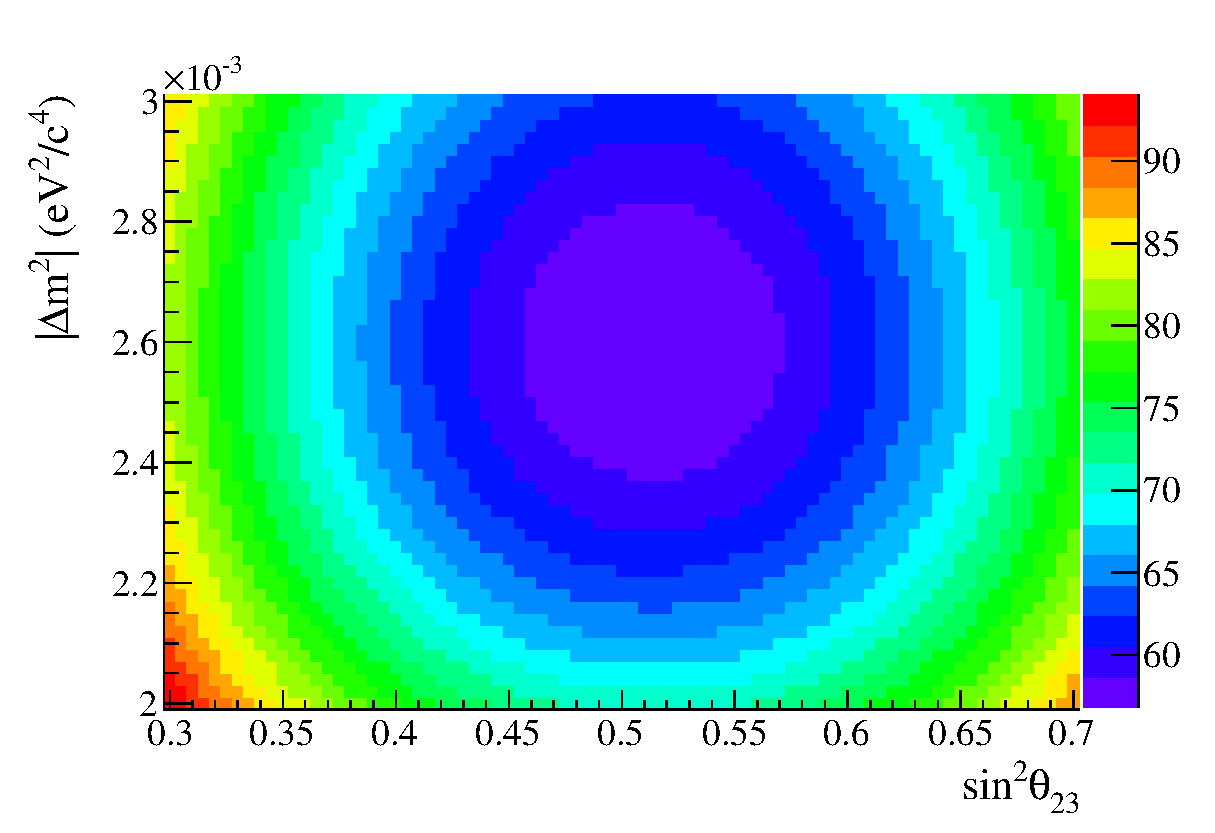
\includegraphics[width=20pc]{./images/prediction/Nsk_1Rmu_disap.eps}
\caption {
  Predicted number of single $\mu$-like ring events,
  as a function of $\sin^{2}\theta_{23}$ and $|\Delta m^{2}|$,
  for an exposure of 3.010$\times$10$^{20}$ POT.
  The number of events was calculated using the BANFF-tuned MC templates.
  2012 PDG values are used for $\sin^{2}\theta_{13}$, $\sin^{2}\theta_{12}$ and $\delta m^{2}$ and $\delta_{CP}$=0.
  The numbers shown were generated assuming the normal hierarchy.
}
\label{fig:Nsk1Rmu_vs_Dmsq_theta23_tunedmc}
\end{minipage}
\hspace{0.06\linewidth}
\begin{minipage}[t]{0.48\linewidth}
\center
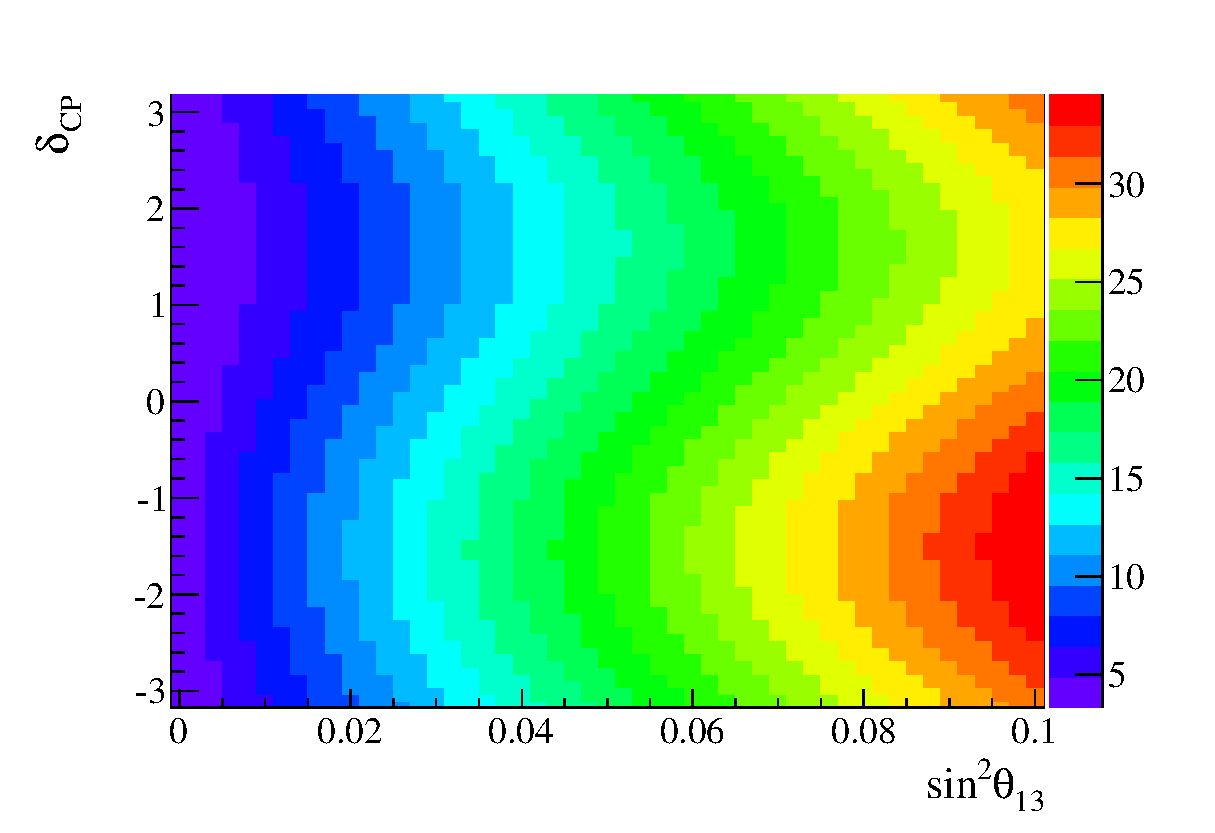
\includegraphics[width=20pc]{./images/prediction/Nsk_1Re_app.eps}
\caption {
  Predicted number of single e-like ring events,
  as a function of $\sin^{2}\theta_{13}$ and $\delta_{CP}$,
  for an exposure of 3.010$\times$10$^{20}$ POT.
  The number of events was calculated using the BANFF-tuned MC templates.
  2012 PDG values are used for $\sin^{2}\theta_{12}$, $|\Delta m^{2}|$ and $\delta m^{2}$,
  while $\sin^{2}\theta_{23}$ was set to 0.5.
  The numbers shown were generated assuming the normal hierarchy.
}
\label{fig:Nsk1Re_vs_dcp_theta13_tunedmc}
\end{minipage}
\end{figure*}


%...........
%
% NSK 1Rmu, 1Re vs osc params typically fixed in stand-alone analyses
%
\begin{figure*}[htb]
\begin{minipage}[t]{0.48\linewidth}
\center
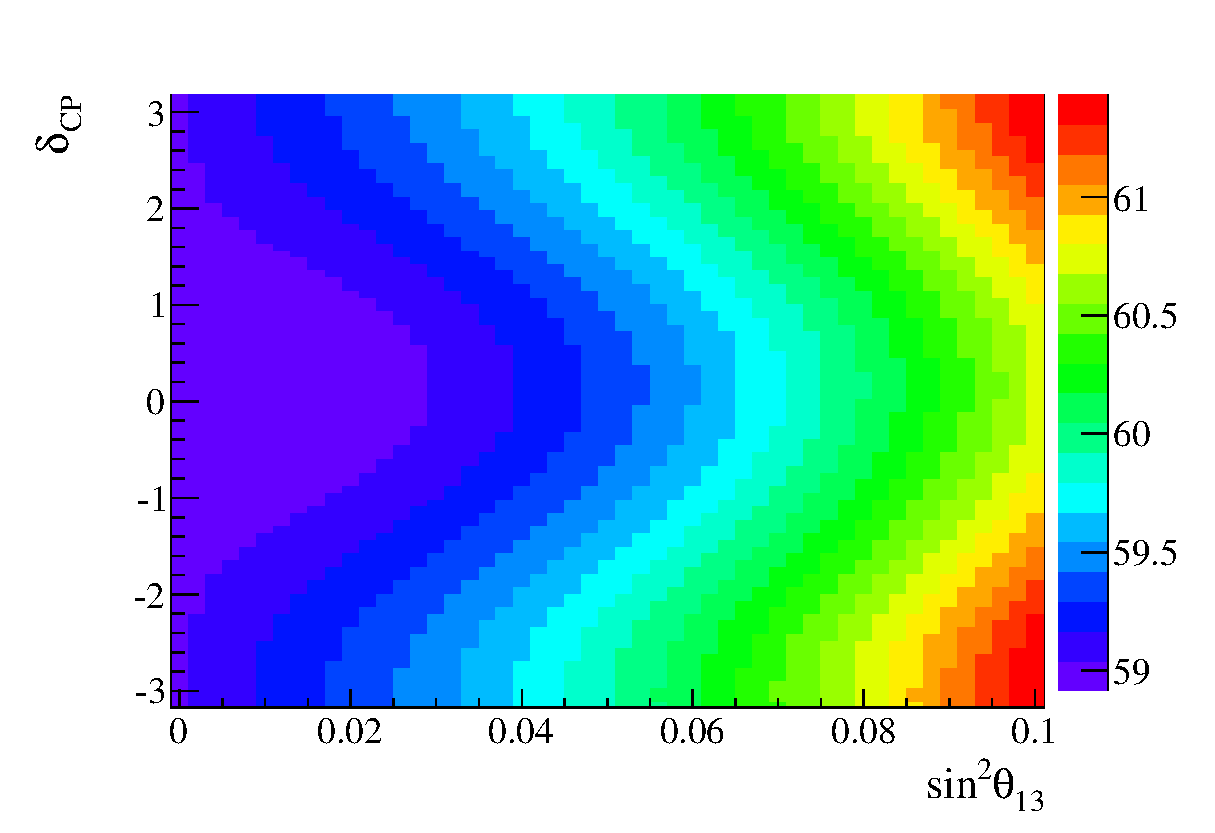
\includegraphics[width=20pc]{./images/prediction/Nsk_1Rmu_app.eps}
\caption {
  Predicted number of single $\mu$-like ring events,
  as a function of $\sin^{2}\theta_{13}$ and $\delta_{CP}$,
  which are typically fixed to constant values by the stand-alone $\nu_{\mu}$-disappearance analysis,
  for an exposure of 3.010$\times$10$^{20}$ POT.
  The number of events was calculated using the BANFF-tuned MC templates.
  2012 PDG values are used for $\sin^{2}\theta_{12}$, $|\Delta m^{2}|$ and $\delta m^{2}$,
  while $\sin^{2}\theta_{23}$ was set to 0.5.
  The numbers shown were generated assuming the normal hierarchy.
}
\label{fig:Nsk1Rmu_vs_dcp_theta13_tunedmc}
\end{minipage}
\hspace{0.06\linewidth}
\begin{minipage}[t]{0.48\linewidth}
\center
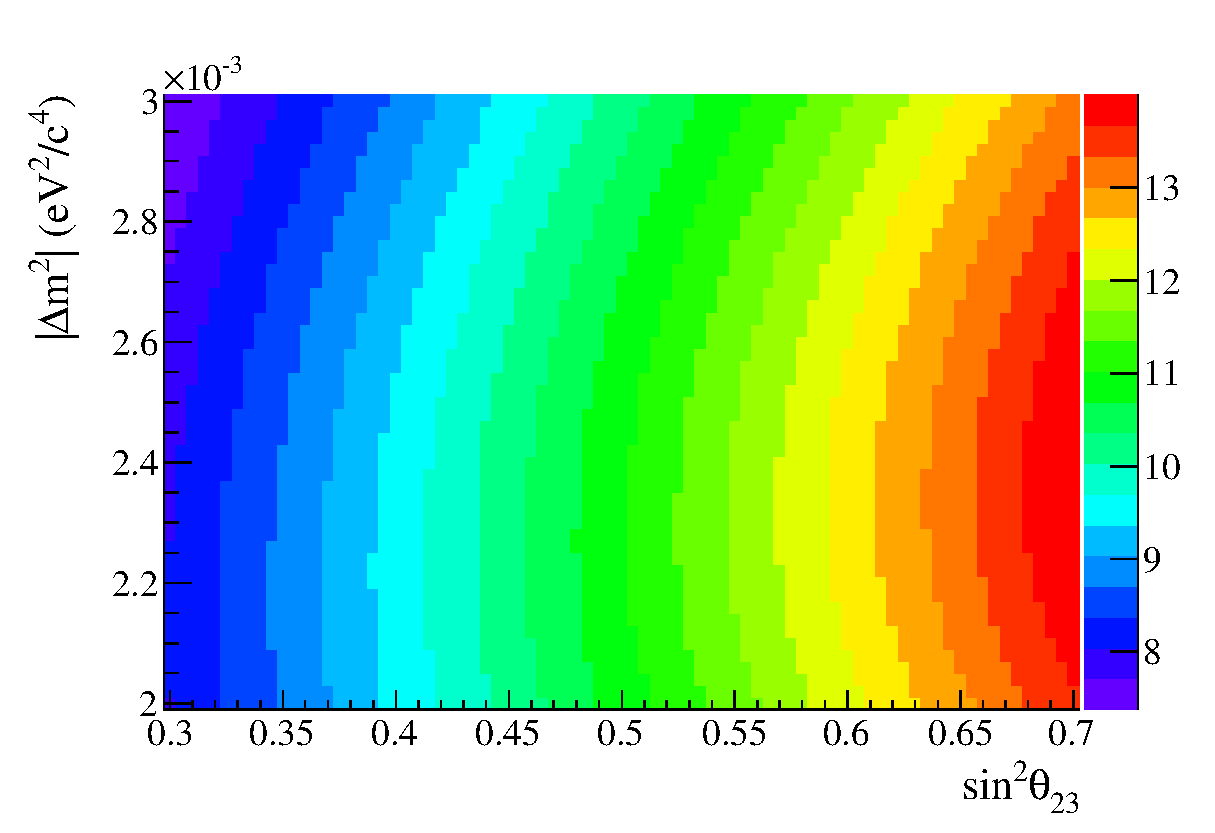
\includegraphics[width=20pc]{./images/prediction/Nsk_1Re_disap.eps}
\caption {
  Predicted number of single e-like ring events,
  as a function of $\sin^{2}\theta_{23}$ and $|\Delta m^{2}|$,
  which are typically fixed to constant values by the stand-alone $\nu_{e}$-appearance analysis,
  for an exposure of 3.010$\times$10$^{20}$ POT.
  The number of events was calculated using the BANFF-tuned MC templates.
  2012 PDG values are used for $\sin^{2}\theta_{13}$, $\sin^{2}\theta_{12}$ and $\delta m^{2}$ and $\delta_{CP}$=0.
  The numbers shown were generated assuming the normal hierarchy.
}
\label{fig:Nsk1Re_vs_Dmsq_theta23_tunedmc}
\end{minipage}
\end{figure*}

%...........
%
% 1Rmu, 1Re spectra - no oscillations
%
\begin{figure*}[htb]
\begin{minipage}[t]{0.48\linewidth}
\center
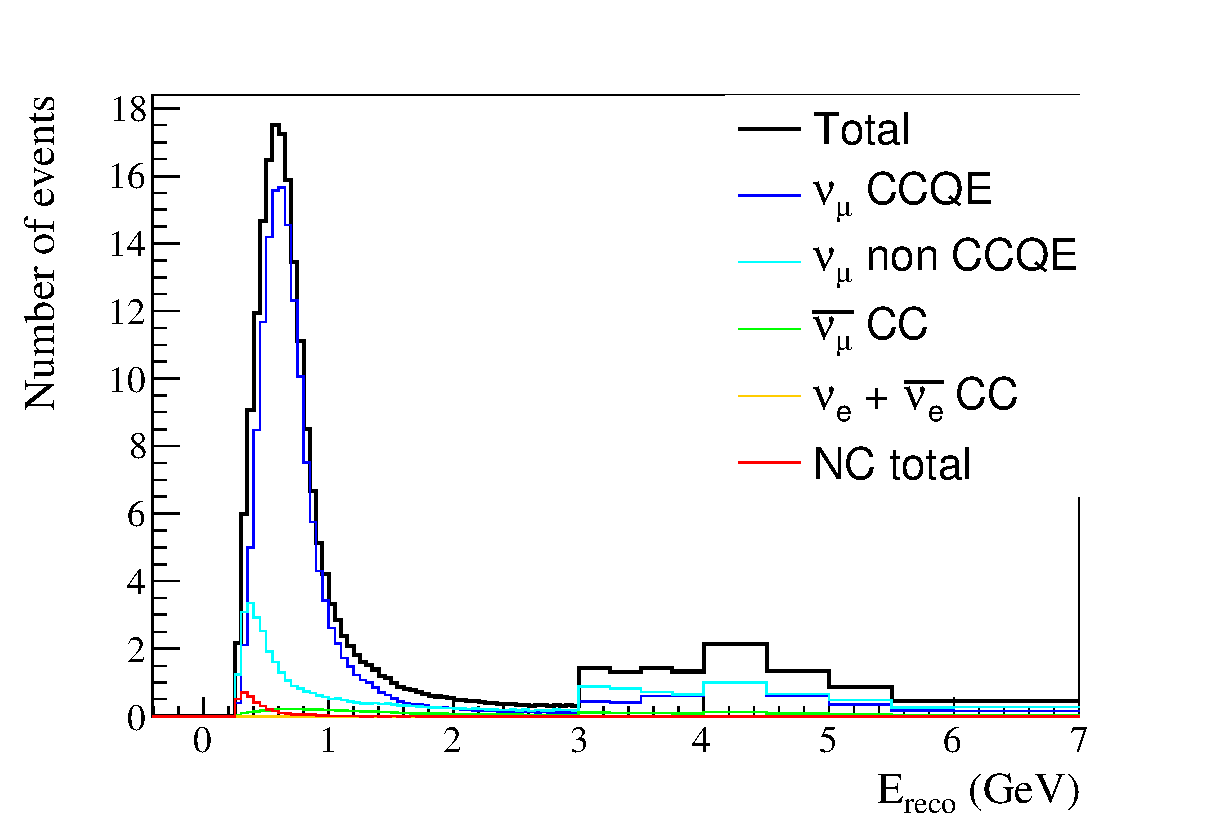
\includegraphics[width=20pc]{./images/prediction/1Rmu_spectrum_no_osc.eps}
\caption {
 Predicted reconstructed-energy spectrum of single $\mu$-like ring events,
 and contributions from various true neutrino reaction modes,
 for no oscillations and
 for an exposure of 3.010$\times$10$^{20}$ POT.
 The 28 components of the spectrum are calculated separately in the actual analysis,
 but, for this plot, are grouped into just 5 categories:
 $\nu_{\mu}$ CCQE, $\nu_{\mu}$ CCnonQE, $\bar{\nu}_{\mu}$ CC, $\nu_{e}$/$\bar{\nu}_{e}$ CC and NC.
 The spectrum was generated using the BANFF-tuned MC templates.
}
\label{fig:1Rmu_spectrum_and_components_no_osc}
\end{minipage}
\hspace{0.06\linewidth}
\begin{minipage}[t]{0.48\linewidth}
\center
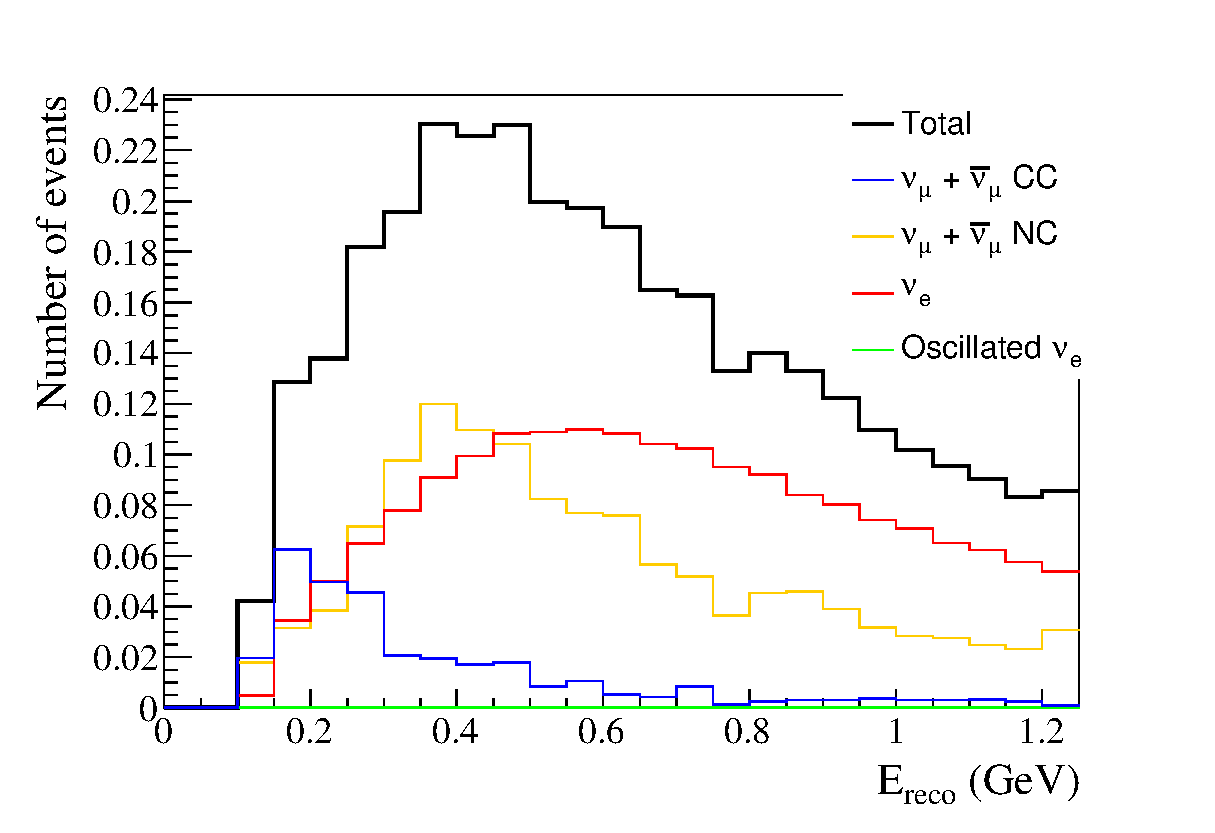
\includegraphics[width=20pc]{./images/prediction/1Re_spectrum_no_osc.eps}
\caption {
Predicted reconstructed-energy spectrum of single e-like ring events,
and contributions from various true neutrino reaction modes,
for no oscillations and
for an exposure of 3.010$\times$10$^{20}$ POT.
The 32 components of the spectrum are calculated separately in the actual analysis,
but, for this plot, are grouped into just four categories: 
$\nu_{\mu}$+$\bar{\nu}_{\mu}$ CC, $\nu_{\mu}$+$\bar{\nu}_{\mu}$ NC, $\nu_{e}$+$\bar{\nu}_{e}$ (intrinsic beam component)
and oscillated $\nu_{e}$.
The spectrum was generated using the BANFF-tuned MC templates.
}
\label{fig:1Re_spectrum_and_components_no_osc}
\end{minipage}
\end{figure*}

%...........
%
% 1Rmu, 1Re spectra - oscillations with typical parameters
%
\begin{figure*}[htb]
\begin{minipage}[t]{0.48\linewidth}
\center
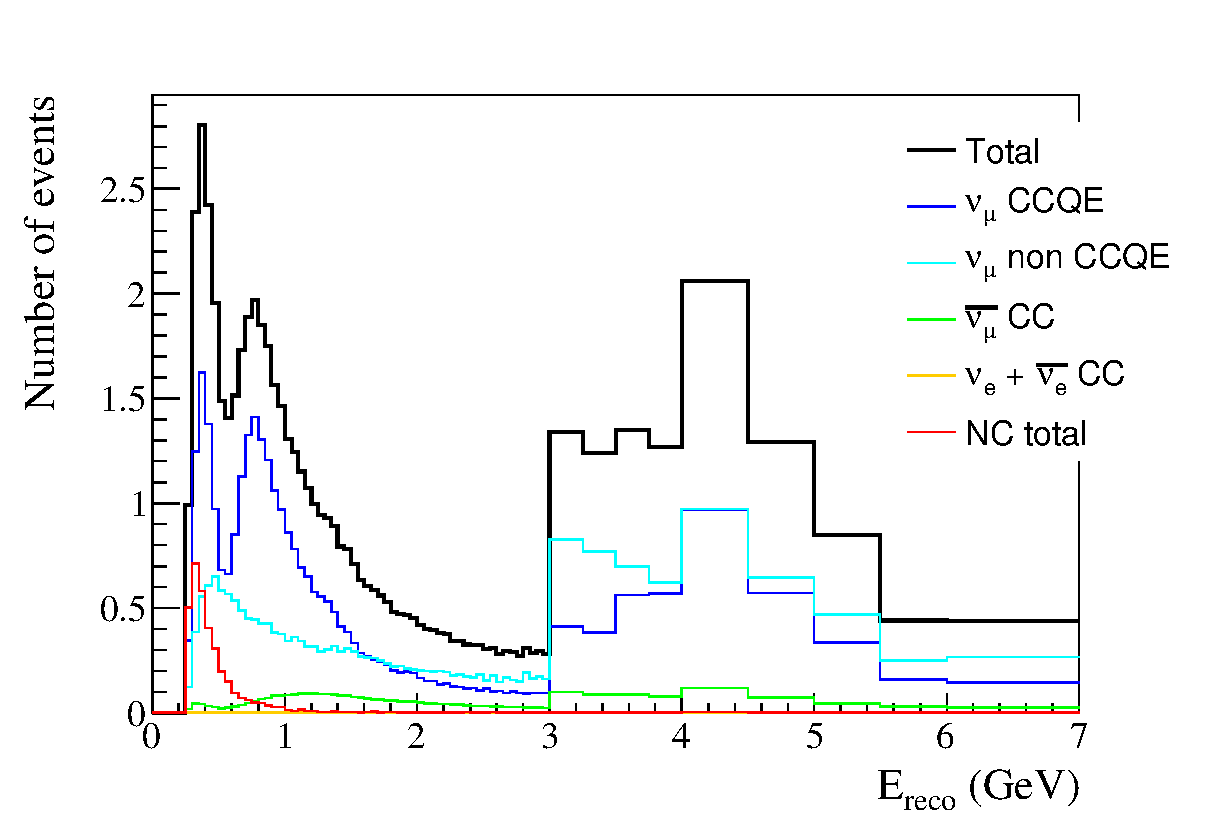
\includegraphics[width=20pc]{./images/prediction/1Rmu_spectrum_PDG.eps}
\caption {
Predicted reconstructed-energy spectrum of single $\mu$-like ring events,
and contributions from various true neutrino reaction modes,
for oscillations with $\sin^{2}\theta_{23}$=0.5 and $|\Delta m^{2}|$=2.4$\times$10$^{-3}$ eV$^{2}$/c$^{4}$
The spectrum was generated using the BANFF-tuned MC templates.
2012 PDG values are used for $\sin^{2}\theta_{13}$, $\sin^{2}\theta_{12}$ and $\delta m^{2}$,
while $\delta_{CP}$=0.
The spectrum shown was generated assuming the normal hierarchy.
Note that the vertical axis is zoomed in by a factor of 4 compared with Fig.\ \ref{fig:1Rmu_spectrum_and_components_no_osc}.
}
\label{fig:1Rmu_spectrum_and_components_default_osc}
\end{minipage}
\hspace{0.06\linewidth}
\begin{minipage}[t]{0.48\linewidth}
\center
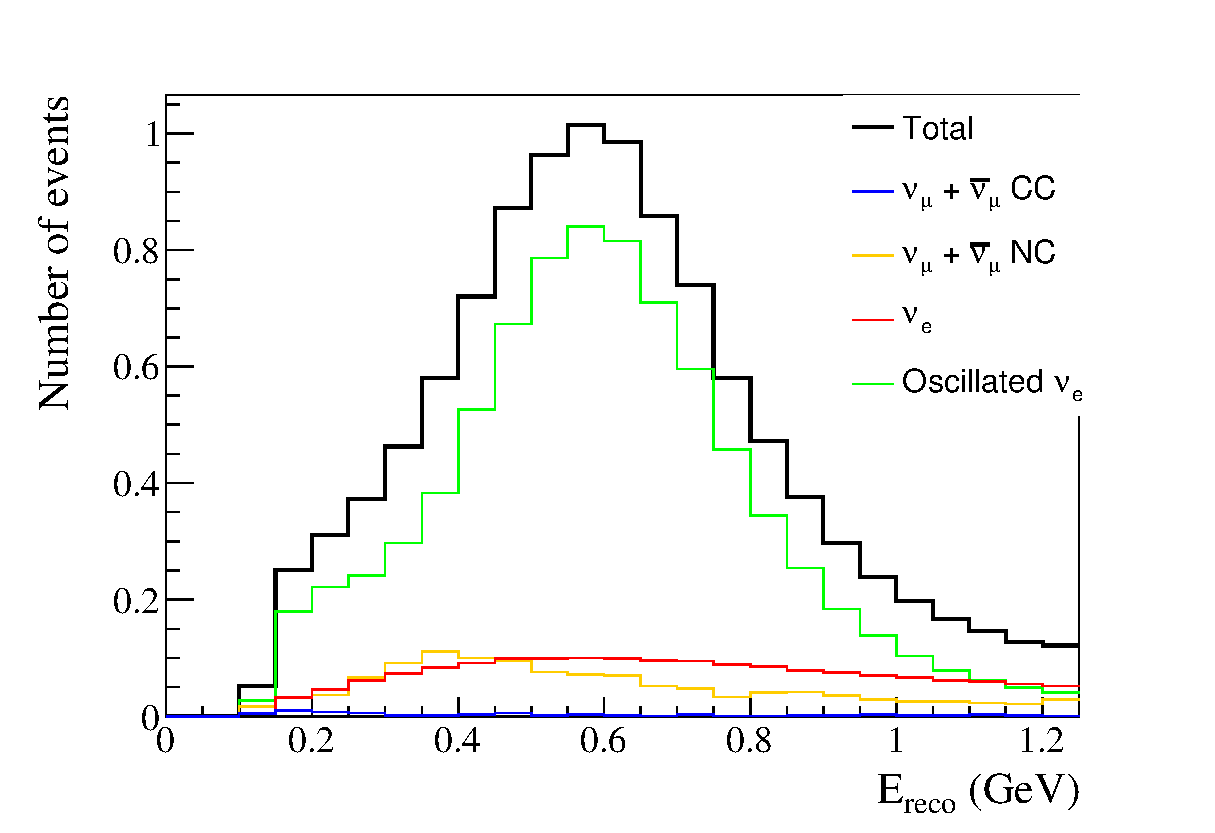
\includegraphics[width=20pc]{./images/prediction/1Re_spectrum_PDG.eps}
\caption {
Predicted reconstructed-energy spectrum of single e-like ring events,
and contributions from various true neutrino reaction modes,
for oscillations with $\sin^{2}\theta_{23}$=0.5, $|\Delta m^{2}|$=2.4$\times$10$^{-3}$ eV$^{2}$/c$^{4}$,
$\sin^{2}\theta_{13}$=0.098 and for an exposure of 3.010$\times$10$^{20}$ POT.
The spectrum was generated using the BANFF-tuned MC templates.
2012 PDG values are used for $\sin^{2}\theta_{12}$ and $\delta m^{2}$,
while $\delta_{CP}$=0.
The spectrum shown was generated assuming the normal hierarchy.
}
\label{fig:1Re_spectrum_and_components_default_osc}
\end{minipage}
\end{figure*}

%...........
%
% tables showing the effect of tunes on nsk and nsk components - no oscillations
%
\begin{table}
\centering
\begin{tabular}{| c || c | c | c || c | c | c | }
\hline  
                                                      & \multicolumn{6}{c|}{$N_{SK}$} \\
\hline  
                                                      & \multicolumn{3}{c||}{ single $\mu$-like ring} & \multicolumn{3}{c|}{ single e-like ring } \\
\hline  
                                                                               & Nominal  & NA61-tuned   & BANFF-tuned  & Nominal    & NA61-tuned   & BANFF-tuned    \\
\hline
Total &                                                                    190.986               &         210.465     &       204.624                 &     2.971      &      3.239        &       3.380           \\
\hline  
$\nu_\mu$ CCQE &                                                      151.820                    &     166.354         &      154.915         &     0.217      &        0.237      &       0.223           \\
$\nu_\mu$ CC 1$\pi$ &                                                             25.718        &       28.880       &         34.955      &   0.060        &    0.066          &        0.083          \\
$\nu_\mu$ CC coherent &                                                         0.898          &      1.005        &       0.950        &      0.0     &       0.0       &         0.0         \\
$\nu_\mu$ CC other &                                                              3.585        &     4.315         &          4.199     &        0.006   &     0.007         &      0.006            \\
$\nu_\mu$/$\nu_\tau$ NC 1$\pi^{+/-}$ ( 1R$\mu$ only)&             1.493               &    1.697          &      1.626         &    -      &      -       &       -          \\
$\nu_\mu$/$\nu_\tau$ NC 1$\pi^{0}$ (1R$_{e}$ only)&                            -     &      -       &      -        &    0.574       &     0.649         &       0.715           \\
$\nu_\mu$/$\nu_\tau$ NC coherent (1R$_{e}$ only)&                              -     &      -       &      -        &      0.193     &          0.218    &        0.208          \\
$\nu_\mu$/$\nu_\tau$ NC other &                                                  1.295         &      1.522        &       1.467        &      0.245     &        0.286      &       0.275           \\
$\bar{\nu}_{\mu}$ CCQE &                                                       4.119           &        4.460      &        3.978       &     0.002      &     0.002         &           0.002       \\
$\bar{\nu}_{\mu}$ CC 1$\pi$ &                                                   1.337          &       1.445       &      1.763         &    0.0004       &       0.0004       &     0.0005             \\
$\bar{\nu}_{\mu}$ CC coherent &                                          0.195                 &        0.211      &      0.203         &     0.0001      &      0.0001        &      0.0001            \\
$\bar{\nu}_{\mu}$ CC other &                                                     0.237         &         0.254     &        0.248       &      0.0     &     0.0         &        0.0          \\
$\bar{\nu}_{\mu}$/$\bar{\nu}_{\tau}$ NC 1$\pi^{+/-}$ (1R$\mu$ only) &    0.080       &    0.092          &      0.090         &    -      &      -       &       -          \\
$\nu_\mu$/$\nu_\tau$ NC 1$\pi^{0}$ (1R$_{e}$ only)&                           -      &      -       &      -        &     0.028      &       0.031       &      0.035            \\
$\nu_\mu$/$\nu_\tau$ NC coherent (1R$_{e}$ only)&                             -      &      -       &      -        &    0.018       &       0.020       &          0.019        \\
$\bar{\nu}_{\mu}$/$\bar{\nu}_{\tau}$ NC other &                                0.073           &       0.079       &        0.078       &   0.014        &     0.015         &        0.015          \\
$\nu_e$ CCQE &                                                            0.016                &       0.017       &        0.016       &     1.114      &        1.180      &           1.134       \\
$\nu_e$ CC 1$\pi$ &                                                       0.009                &        0.010      &        0.013       &      0.352     &       0.377       &         0.505         \\
$\nu_e$ CC coherent &                                                0.0004                     &     0.0004         &      0.0004         &      0.005     &      0.005        &          0.005        \\
$\nu_e$ CC other &                                                               0.003         &      0.003        &         0.003      &     0.028      &      0.030        &          0.029        \\
$\nu_e$ NC 1$\pi^{+/-}$ (1R$\mu$ only) &                            0.042            &      0.050        &      0.049         &    -      &      -       &      -           \\
$\nu_\mu$/$\nu_\tau$ NC 1$\pi^{0}$ (1R$_{e}$ only)&                           -      &      -       &      -        &      0.015     &    0.018          &        0.020          \\
$\nu_\mu$/$\nu_\tau$ NC coherent (1R$_{e}$ only)&                             -      &      -       &      -        &     0.004      &         0.005     &        0.005          \\
$\nu_e$ NC other &                                                                 0.005       &      0.057        &       0.057        &     0.009      &      0.010        &           0.010       \\
$\bar{\nu}_{e}$ CCQE &                                                        0.0008            &     0.0008         &       0.0008        &     0.052      &     0.052         &          0.051        \\
$\bar{\nu}_{e}$ CC 1$\pi$ &                                                            0.0006   &       0.0006       &      0.0007         &      0.021     &      0.021        &           0.029       \\
$\bar{\nu}_{e}$ CC coherent &                                                0.00007             &      0.00007        &        0.00007       &    0.004       &      0.004        &      0.004            \\
$\bar{\nu}_{e}$ CC other &                                                             0.0002   &        0.0002      &       0.0002        &    0.002       &    0.002          &          0.002        \\
$\bar{\nu}_{e}$ NC 1$\pi^{+/-}$ (1R$\mu$ only) &                0.006                &  0.006            &        0.006       &    -      &      -       &      -           \\
$\nu_\mu$/$\nu_\tau$ NC 1$\pi^{0}$ (1R$_{e}$ only)&                           -      &      -       &      -        &   0.002        &      0.002        &        0.002          \\
$\nu_\mu$/$\nu_\tau$ NC coherent (1R$_{e}$ only)&                             -      &      -       &      -        &      0.0009     &           0.0009   &         0.0009         \\
$\bar{\nu}_{e}$ NC other &                                                                &    0.006          &    0.006           &     0.001      &    0.001          &       0.001           \\
Oscillated $\nu_e$ CCQE &                                                             0          &          0    &        0       &       0    &          0    &         0         \\
Oscillated $\nu_e$ CC 1$\pi$ &                                                         0         &           0   &         0      &        0   &          0    &          0        \\
Oscillated $\nu_e$ CC coherent &                                                       0         &           0   &         0      &        0   &         0     &          0        \\
Oscillated $\nu_e$ CC other &                                                                0   &             0 &              0 &           0&            0  &              0    \\
\hline
\end{tabular}
\caption{
  Calculated numbers of single $\mu$-like ring and single e-like ring events without oscillations using the nominal MC templates, 
  the NA61-tuned MC templates and the BANFF-tuned MC templates.
  The total numbers of events and the numbers of events from each mode considered in this analysis are shown.
  These numbers were calculated for an exposure of 3.010$\times$10$^{20}$ POT.
  Note that different NC MC templates are used for predicting the number of single $\mu$-like ring and single e-like ring events.
}
\label{tab:nsk_nominal_x3_no_osc}
\end{table}


%...........
%
% tables showing the effect of tunes on nsk and nsk components - default oscillations
%
\begin{table}
\centering
\begin{tabular}{| c || c | c | c || c | c | c | }
\hline  
                                                      & \multicolumn{6}{c|}{$N_{SK}$} \\
\hline  
                                                      & \multicolumn{3}{c||}{ single $\mu$-like ring} & \multicolumn{3}{c|}{ single e-like ring } \\
\hline  
                                                                               & Nominal  & NA61-tuned   & BANFF-tuned  & Nominal    & NA61-tuned   & BANFF-tuned    \\
\hline
Total &                      54.264                                                             &  60.939            &  59.799             &  10.036         &  10.961            &  11.012                \\
\hline
$\nu_\mu$ CCQE &                                                                  30.926	&	34.183       &  30.962  	   &	0.028	    &	0.031		&	0.028		\\
$\nu_\mu$ CC 1$\pi$ &                                                             13.198	&	15.137       &  17.572  	   &	0.021	    &	0.023		&	0.029		\\
$\nu_\mu$ CC coherent &                                                            0.377	&	 0.434       &   0.412  	   &	0.000	    &	0.000		&	0.000		\\
$\nu_\mu$ CC other &                                                               3.210	&	 3.888       &   3.796  	   &	0.003	    &	0.003		&	0.003		\\
$\nu_\mu$/$\nu_\tau$ NC 1$\pi^{+/-}$ (1R$\mu$-like only)&                     1.492	&	 1.697       &   1.626  	   &	-      &      -       &       - 	 \\
$\nu_\mu$/$\nu_\tau$ NC 1$\pi^{0}$ (1R$_{e}$ only)&                            -     &      -       &      -        &   0.574	  &	0.649	      & 0.715		      \\
$\nu_\mu$/$\nu_\tau$ NC coherent (1R$_{e}$ only)&                              -     &      -       &      -        &   0.193	  &	0.218	      & 0.208		      \\
$\nu_\mu$/$\nu_\tau$ NC other &                                                    1.294       &	1.522	   &	1.466		&	0.248      &	0.286   	 &	0.274   	   \\
$\bar{\nu}_{\mu}$ CCQE &                                                           2.071       &	2.244	   &	1.936		&	0.0006      &	 0.0007 	  &	 0.0006 	    \\
$\bar{\nu}_{\mu}$ CC 1$\pi$ &                                                      0.976       &	1.053	   &	1.254		&	0.0002     &	0.0002  	 &	0.0002  	   \\
$\bar{\nu}_{\mu}$ CC coherent &                                                    0.107       &	0.116	   &	0.111		&	0.00007    &	0.00007 	 &	0.00007 	   \\
$\bar{\nu}_{\mu}$ CC other &                                                       0.211       &	0.226	   &	0.221		&	0.000      &	0.000   	 &	0.000   	   \\
$\bar{\nu}_{\mu}$/$\bar{\nu}_{\tau}$ NC 1$\pi^{+/-}$ (1R$\mu$ only) &    0.084       &	0.092	   &	0.090		&    -      &	   -	   &	   -	      \\
$\nu_\mu$/$\nu_\tau$ NC 1$\pi^{0}$ (1R$_{e}$ only)&                           -      &      -       &      -        &   0.028	  &	0.030	      & 0.034		      \\
$\nu_\mu$/$\nu_\tau$ NC coherent (1R$_{e}$ only)&                             -      &      -       &      -        &   0.018	  &	0.019	      & 0.018		      \\
$\bar{\nu}_{\mu}$/$\bar{\nu}_{\tau}$ NC other &                                    0.073 	&	0.079        &  0.077   	   &	0.013	    &	0.015		&	0.014		\\
$\nu_e$ CCQE &                                                                     0.014 	&	0.015        &  0.014   	   &	1.025	    &	1.085		&	1.042		\\
$\nu_e$ CC 1$\pi$ &                                                                0.008 	&	0.009        &  0.012   	   &	0.331	    &	0.355		&	0.476		\\
$\nu_e$ CC coherent &                                                              0.0004	&	0.0004       &  0.0003  	   &	0.004	    &	0.004		&	0.004		\\
$\nu_e$ CC other &                                                                 0.002 	&	0.003        &  0.002   	   &	0.026	    &	0.029		&	0.028		\\
$\nu_e$ NC 1$\pi^{+/-}$ (1R$\mu$ only) &                                 0.042 	&	0.048        &  0.048   	   &	 -     &      -       &       - 	 \\
$\nu_\mu$/$\nu_\tau$ NC 1$\pi^{0}$ (1R$_{e}$ only)&                           -      &      -       &      -        &   0.015	  &	0.017	      & 0.020		      \\
$\nu_\mu$/$\nu_\tau$ NC coherent (1R$_{e}$ only)&                             -      &      -       &      -        &   0.004	  &	0.005	      & 0.004		      \\
$\nu_e$ NC other &                                                                0.049  	 &	0.057          & 0.057   	      & 0.009	       &	0.010	   &	0.010		   \\
$\bar{\nu}_{e}$ CCQE &                                                            0.0008 	 &	0.0007         &0.0007  	      & 0.048	       &	0.048	   &	0.047		   \\
$\bar{\nu}_{e}$ CC 1$\pi$ &                                                       0.0006 	 &	0.0005         &0.0007  	      & 0.020	       &	0.020	   &	0.027		   \\
$\bar{\nu}_{e}$ CC coherent &                                                     0.00007	 &	0.00007        &0.00007 	      & 0.003	       &	0.003	   &	0.003		   \\
$\bar{\nu}_{e}$ CC other &                                                        0.0002 	 &	0.0002         &0.0002  	      & 0.002	       &	0.001	   &	0.001		   \\
$\bar{\nu}_{e}$ NC 1$\pi^{+/-}$ (1R$\mu$ only) &                        0.006  	 &	0.005          &0.005   	      &    -	  &	 -	 &	 -	    \\
$\nu_\mu$/$\nu_\tau$ NC 1$\pi^{0}$ (1R$_{e}$ only)&                           -      &      -       &      -        &  0.001 	   &	0.001   	&	0.002   	 \\
$\nu_\mu$/$\nu_\tau$ NC coherent (1R$_{e}$ only)&                             -      &      -       &      -        &  0.0009	   &	0.0009  	&	0.0009  	 \\
$\bar{\nu}_{e}$ NC other &                                                        0.006  	 &	0.005        & 	0.006       &	0.001	     &  0.001		 &	0.001		 \\
Oscillated $\nu_e$ CCQE &                                                         0.080  	       &0.088   	    &	0.083   	  &	6.378	   &	6.965	       &	6.567	       \\
Oscillated $\nu_e$ CC 1$\pi$ &                                                    0.025  	       &0.026   	    &	0.034   	  &	0.996	   &	1.090	       &	1.406	       \\
Oscillated $\nu_e$ CC coherent &                                                  0.002  	       &0.002   	    &	0.001   	  &	0.020	   &	0.022	       &	0.021	       \\
Oscillated $\nu_e$ CC other &                                                     0.0006 	       &0.0006  	    &	0.0006  	  &	0.014	   &	0.015	       &	0.014	       \\
\hline
\end{tabular}
\caption{
  Calculated numbers of single $\mu$-like ring and single e-like ring events with oscillations
  using the nominal MC templates, the NA61-tuned MC templates and the BANFF-tuned MC templates.
  The total numbers of events and the numbers of events from each mode considered in this analysis are shown.
  These numbers were calculated for an exposure of 3.010$\times$10$^{20}$ POT 
  and oscillations with $\delta_{CP}$=0, $\sin^{2}\theta_{13}$=0.025, $\sin^{2}\theta_{23}$=0.5 and $|\Delta m^{2}|$=2.4$\times$10$^{-3}$ eV$^{2}$/c$^{4}$.
  The 2012 PDG parameters are used for $\sin^{2}\theta_{12}$ and $\delta m^{2}$.
  The normal hierarchy is assumed.
  Note that different NC MC templates are used for predicting the number of single $\mu$-like ring and single e-like ring events.
}
\label{tab:nsk_nominal_x3_default_osc}
\end{table}









